\documentclass[11pt,a4paper]{article}

\usepackage[english]{babel}
\usepackage[T1]{fontenc}
\usepackage[utf8]{inputenc}
\usepackage{graphicx}
\graphicspath{{../Figs/}}
\usepackage{float}
\usepackage{subcaption}
\usepackage[font=footnotesize,labelfont={sf,bf},textfont=sf,width=\textwidth]{caption}
\usepackage[margin=2cm]{geometry}
\usepackage[plainpages=false,pdfpagelabels,hypertexnames=false]{hyperref}
\usepackage[usenames,dvipsnames]{xcolor}
\usepackage{mathtools}
\usepackage[makeroom]{cancel}
\usepackage[separate-uncertainty=true, multi-part-units=single]{siunitx}
\usepackage{booktabs}
\usepackage{physics}
\usepackage[title]{appendix}

\title{\bfseries\textsc{Hall effect in semiconductors}}
\author{
Michele Masini\\ \small\texttt{\href{mailto:michele.masini@uni-ulm.de}{michele.masini@uni-ulm.de}}\and
Iyán Méndez Veiga\\ \small\texttt{\href{mailto:iyan.mendez-veiga@uni-ulm.de}{iyan.mendez-veiga@uni-ulm.de}}
}
\date{\today}

\begin{document}
\maketitle

\section{Introduction}
In this experiment, we determine the carrier density $p$ and the mobility $\mu$ of a p-type Silicon semiconducting sample doped with Boron. We determine these quantities as a function of the temperature in the range \SIrange{80}{300}{\kelvin}.

In order to obtain the carrier density we use the Hall effect. Once the Hall coefficient is known, mobility is computed by measuring the resistivity $\rho$ of the sample. Since preparing a «Hall bar» is very time consuming, resistivity is measured by means of the van der Pauw method~\cite{vdP}.

\section{Theory}

Electrons in a semiconductor interact both with the positively charged atomic nuclei and with other electrons. This rather complex interaction can be condensed in an effective lattice-periodic potential $V(\vec{r})$. Hence, time-independent Schrödinger equation can be written in this way:

\begin{equation}\label{eq:Schr}
\left[-\frac{\hbar^2}{2m}\laplacian + V(\vec{r})\right]\psi(\vec{r})=E\psi(\vec{r})\,,
\end{equation}
where the eigenvalues $E$ are the possible energies of the electrons, and $\psi(\vec{r})$ the corresponding eigenfunctions:

\begin{equation*}
\psi(\vec{r})=\psi_{\vec{k}}(\vec{r})=u_{\vec{k}}(\vec{r})\exp\left(i\vec{k}\vdot\vec{r}\right)
\end{equation*}

These eigenfunctions are called \emph{Bloch waves}, where $u_{\vec{k}}(\vec{r})$ is a lattice-periodic function and $\vec{k}$ is a quantized wavevector, which indexes the solutions of the Schrödinger equation.

The possible energies $E$ for different semiconductors are usually drawn in a band-structure plot, which shows the values of $E(\vec{k})$ in particular straight lines in the $\vec{k}$ space connecting symmetry points in the first Brillouin zone. In Figure \ref{fig:silicon_band_structure}, the band structure of Silicon is shown.

\begin{figure}[ht]
\centering
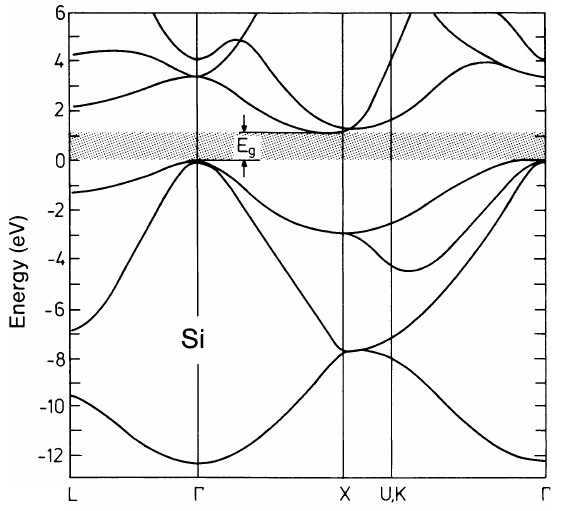
\includegraphics[width=0.5\textwidth]{Si_band_structure}
\caption{Calculated band structure of Silicon. Si is an indirect semiconductor because the maximum of the valence band and the minimum of the conduction bands are located at different positions in $\vec{k}$ space.\cite{ibach2009solid}}
\label{fig:silicon_band_structure}
\end{figure}

Semiconductors are characterized by the existence of a band gap $E_g$ between the valence and conduction band, where there are no allowed energies, and thus no electronic states exist. Semiconductors have a second property in common: at \SI{0}{\kelvin}, the valence band is completely occupied and the conduction band is completely empty.

At room temperature, Silicon has a band gap of \SI{1.12}{\electronvolt}. This gap increases a bit at \SI{0}{\kelvin} becoming \SI{1.17}{\electronvolt}.

In many cases, electrons in semiconductors can be treated as free particles by replacing the scalar electron mass $m$ by a tensor $\hat{m}$ called the \emph{effective mass tensor}, which includes the effect of the periodic potential $V(\vec{r})$. The components of the inverse of this tensor are given by:

\begin{equation}\label{eq:mass_tensor}
\hat{m}_{ij}^{-1}=\frac{1}{\hbar^2}\pdv[2]{E(\vec{k})}{k_i}{k_j}
\end{equation}

This definition may look artificial but it is the natural choice if we do a Taylor expansion of the energy function up to the second order:

\begin{equation}\label{eq:dispersion_energy}
E(\vec{k})=\underbrace{E(0)}_\text{=0}+\underbrace{\vec{\nabla}E|_{k=0}\vdot \vec{k}}_\text{=0}+\frac{1}{2}\vec{k}^t\cdot\pdv[2]{E}{k_i}{k_j}\cdot\vec{k}+\ldots\simeq\frac{1}{2}\vec{k}^t\cdot\pdv[2]{E}{k_i}{k_j}\cdot\vec{k}
\end{equation}

Definition \eqref{eq:mass_tensor} is even more clear if we rewrite the energy of a free particle in the following way:

\begin{equation*}
\frac{\hbar^2k^2}{2m}=\frac{\hbar^2}{2}\vec{k}^t\left(\frac{1}{m}\right)\vec{k}=\frac{\hbar^2}{2}\vec{k}^t\hat{m}^{-1}\vec{k}\,,
\quad\text{where}\;\hat{m}^{-1}=
\begin{pmatrix*}
1/m & 0 & 0 \\
0 & 1/m & 0 \\
0 & 0 & 1/m
\end{pmatrix*}
\end{equation*}

Around the conduction band minimum, $\hat{m}^{-1}$ can be diagonalized and the energy dispersion in parabolic approximation is given by the following expression using \eqref{eq:mass_tensor} and \eqref{eq:dispersion_energy}:

\begin{equation}\label{eq:energy_dispersion}
E(\vec{k})=\frac{\hbar^2}{2}\vec{k}^t\vdot\hat{m}_{ij}^{-1}\vdot\vec{k}=\frac{\hbar^2}{2}\left(\frac{1}{m_x}k_x^2+\frac{1}{m_y}k_y^2+\frac{1}{m_z}k_z^2\right)
\end{equation}

It is important to note that the three effective masses ($m_x$, $m_y$ and $m_z$) are, in general, different. However, in direct semiconductors such as Gallium arsenide, i.e. those whose valence band maximum and conduction band minimum are both located at the same point in $\vec{k}$ space, the masses are all equal and the constant energy surfaces are spheres as shown in Figure \ref{fig:energy_surfaces}.

\begin{figure}[ht]
\centering
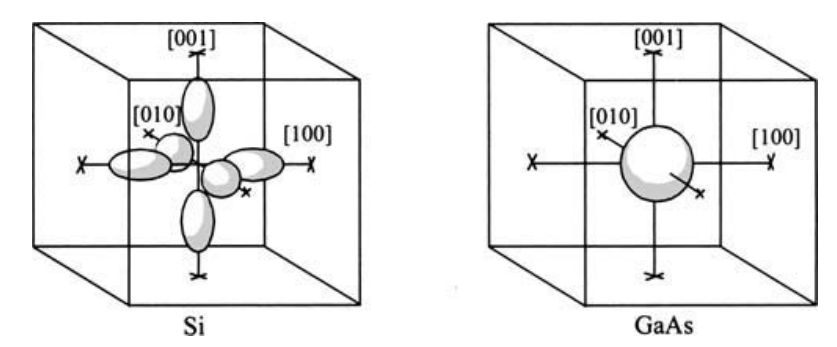
\includegraphics[width=0.6\textwidth]{energy_surfaces}
\caption{Shapes of constant-energy surfaces for electrons in Si and GaAs.\cite{sze2006physics}}
\label{fig:energy_surfaces}
\end{figure}

In the case of Silicon, since it is an indirect semiconductor, the shift of the conduction minimum in $\vec{k}$ space has to be included in equation \eqref{eq:energy_dispersion} and this leads to ellipsoids as constant energy surfaces as shown in Figure \ref{fig:energy_surfaces} instead of spheres. The effective mass along the symmetry axis is called longitudinal mass $m_l$ and the one perpendicular to the symmetry axis is called transverse mass $m_t$.

As mentioned before, expression \eqref{eq:energy_dispersion} is only valid in the vicinity of the conduction band minimum. The structure of the valence band maximum is more complicated than what it looks in Figure \ref{fig:silicon_band_structure}. Besides the two valence bands with different curvatures which can be seen already in that figure, there exists another valence band at point $\Gamma$, i.e. the center of the Brillouin zone, which is split off slightly from the other two as shown in Figure \ref{fig:light_heavy_holes} by $\Delta = \SI{0.044}{\electronvolt}$ in the case of the Silicon.

In the parabolic approximation one can identify three different effective masses for the holes at $\Gamma$ which contribute to charge transport. One speaks of heavy holes and light holes with masses $m_{hh}$ or $m_{lh}$, corresponding to the different band curvatures. The holes of the split-off band are called split-off holes and their mass is denoted by $m_{soh}$.

\begin{figure}[ht]
\centering
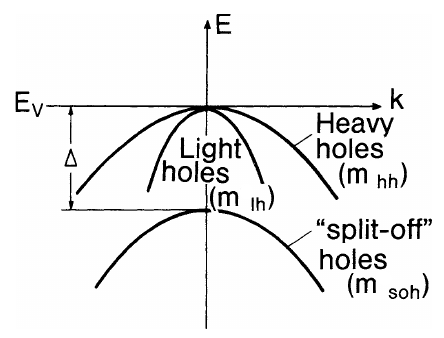
\includegraphics[width=0.4\textwidth]{light_heavy_holes}
\caption{Qualitative band structure for Si in the vicinity of the maximum of the valence band. Valence bands of the heavy and light holes ($hh$ and $lh$) are degenerate at $\vec{k}=0=\Gamma$. There exists a third valence band shifted a bit down due to spin-orbit interactions.\cite{ibach2009solid}}
\label{fig:light_heavy_holes}
\end{figure}

Moreover, the effective mass tensor cannot be diagonalized at this point, and therefore equation \eqref{eq:energy_dispersion} is not valid. Alternatively, a three-parameter expression can be written for the energy dispersion:

\begin{equation}\label{eq:energy_dispersion_alt}
E(\vec{k})_\pm=\frac{\hbar^2}{2m_0}\left[Ak^2\pm\sqrt{B^2k^4+C^2(k_x^2k_y^2+k_y^2k_z^2+k_z^2k_x^2)}\,\right]\,,
\end{equation}
where $A$, $B$ and $C$ are the parameters and $m_0$ the invariant mass of the electron. The $E_+$ corresponds to the heavy holes and $E_-$ to the light holes.

There are two types of semiconductors: intrinsic and extrinsic. The number of holes in intrinsic semiconductors is equal to the number of electrons in the conduction band. In other words, electrons in the conduction band and holes in the valence band exclusively arise from electronic transitions between the valence and the conduction band. This phenomenon can happen thermally or induced by the absorption of light. The number of electrons or holes of a semiconductor can be modified by adding electrically active impurities. These are called extrinsic semiconductors. The doping elements are deliberately chosen in such a way that either they have five electrons in their valence band, or they have just three. When impurities have one more electron than needed for the $sp^3$ binding with the semiconductor element, for example Silicon doped with Phosphor, the extrinsic semiconductor is said to be a n-doped semiconductor and the impurity to be a donor. On the other hand, when impurities have one electron less, for example Silicon doped with Boron, the extrinsic semiconductor is said to be a p-doped semiconductor and the impurity an acceptor. Figure \ref{fig:extrinsic_semiconductors} shows both types of Si extrinsic semiconductors.

\begin{figure}[ht]
\centering
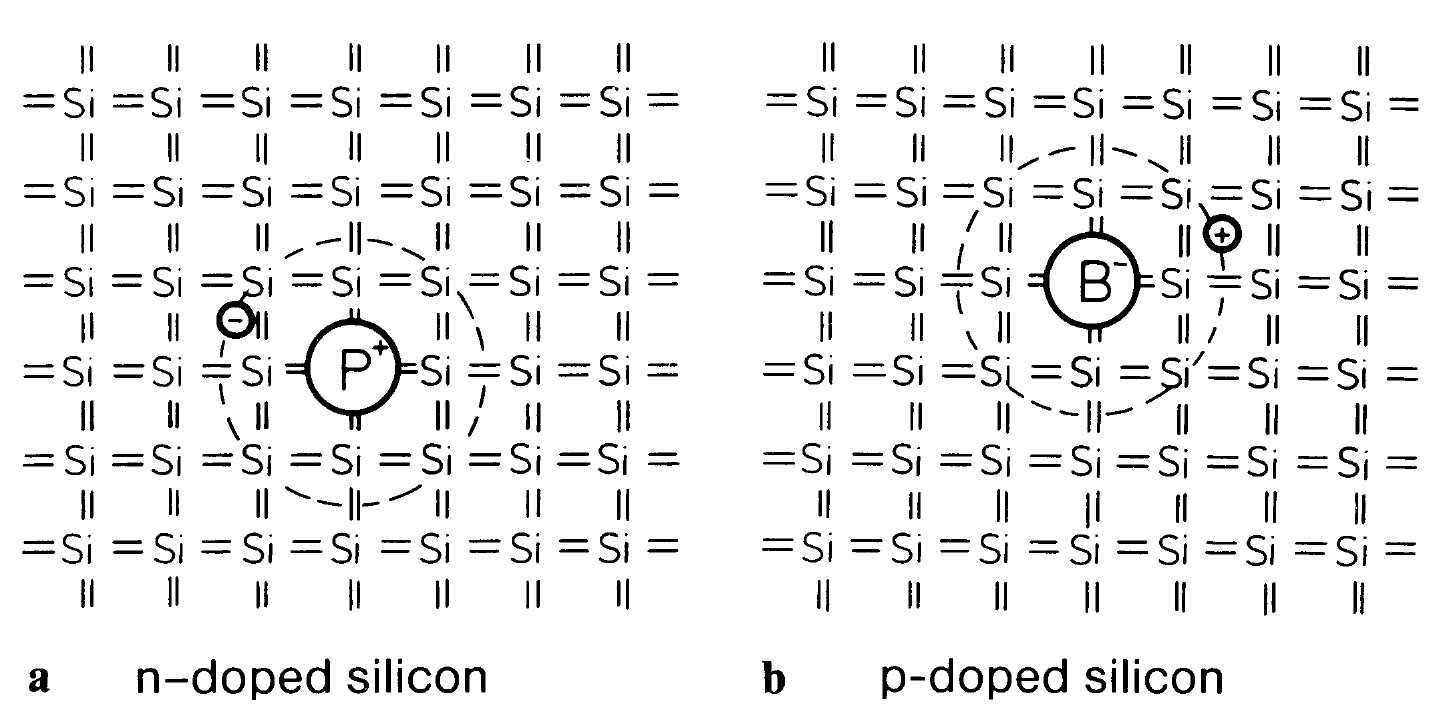
\includegraphics[width=0.6\textwidth]{extrinsic_semiconductors}
\caption{Schematic representation of the effect of a donor (a) and an acceptor (b) in a Silicon lattice. Note that the lattice constant and the radius of the defect center are not drawn to scale. In reality the first Bohr radius of the «impurity orbit» is about ten times as large as the lattice parameter.\cite{ibach2009solid}}
\label{fig:extrinsic_semiconductors}
\end{figure}

The existence of the band gap $E_g$ in semiconductors makes the carrier densities $n$ (electrons) and $p$ (holes) very dependent on temperature. The occupation of electronic states is governed by the Fermi-Dirac distribution:

\begin{equation}\label{eq:Fermi-Dirac}
f(E,T)=\frac{1}{1+\exp\left(\frac{E-E_\text{F}}{k_BT}\right)}\,,
\end{equation}
where $E_\text{F}$ is the Fermi energy, i.e. the limiting energy that separates occupied from unoccupied states at $T=\SI{0}{\kelvin}$, and $k_B$ the Boltzmann constant. But since in our case the charge carriers are holes, our distribution will be $1-f(E,T)$.

Let us call $D_V(E)$ the density of states in the valence band and $E_V$ the valence band edge. Then, we can write the hole density as:

\begin{equation}\label{eq:hole_density}
p=\int_{-\infty}^{E_V}D_V(E)\big[1-f(E,T)\big]\,dE
\end{equation}

The density of states of the valence band can be written in the parabolic approximation:

\begin{equation*}
D_V(E)=\frac{\sqrt{2}}{2\pi^2\hbar^3}\left(m_{lh}^{3/2}+m_{hh}^{3/2}\right)\sqrt{E_V-E}\equiv\frac{\sqrt{2m_{dh}^3}}{2\pi^2\hbar^3}\sqrt{E_V-E}\,,
\end{equation*}
where $m_{dh}=(m_{lh}^{3/2}+m_{hh}^{3/2})^{2/3}$ is the effective density-of-states mass for holes expressed in terms of the masses of heavy and light holes mentioned before.

Defining the effective density of states in the valence band as:

\begin{equation}\label{eq:Nv}
N_V=\frac{2\left(2\pi\,m_{dh}\,k_BT\right)^{3/2}}{h^3}\,,
\end{equation}
the hole density $p$ calculated from integral \eqref{eq:hole_density} can be written:

\begin{equation}\label{eq:p}
p=\frac{2\,N_V}{\sqrt{\pi}}F_{1/2}\!\left(\frac{E_V-E_F}{k_BT}\right)\,,
\end{equation}
where $F_{1/2}(\frac{E_V-E_F}{k_BT})$ denotes the following Fermi-Dirac integral:

\begin{equation*}
F_{1/2}\!\left(\frac{E_V-E_F}{k_BT}\right)\equiv F_{1/2}(\eta_F)=\int_{-\infty}^{E_V}\frac{\sqrt{(E_V-E)/k_BT}}{1+\exp\left[(E_F-E)/k_BT\right]}\frac{dE}{k_BT}=\int_{-\infty}^0\frac{\sqrt{\eta}}{1+\exp(\eta-\eta_F)}d\eta\,,
\end{equation*}
where in the last step the following change of variables was made:
\begin{equation*}
\eta\equiv\frac{E_V-E}{k_BT}\quad,\quad\eta_F\equiv\frac{E_V-E_F}{k_BT}
\end{equation*}

When $k_BT\ll E-E_F$, Fermi-Dirac statistics can be replaced by Boltzmann statistics. In particular, when $k_BT\ll E_F-E_V$ equation \eqref{eq:p} simplifies to:

\begin{equation}\label{eq::p}
p=N_V\exp\left(-\frac{E_F-E_V}{k_BT}\right)
\end{equation}

As mention in the introduction, our sample is a p-type Silicon semiconductor doped with Boron. This means that a concentration $N_A^-$ of ionized acceptors has been added to the material. This concentration can be expressed as:

\begin{equation}\label{eq::Na-}
N_A^-=\frac{N_A}{1+4\exp\left(\frac{E_A-E_F}{k_BT}\right)}\,,
\end{equation}
where $N_A$ is the total concentration of acceptors and $E_A$ the energy of bound acceptor holes.

The Fermi level adjusts itself such that the material respects the neutrality of charge, i.e. $p=n+N_A^-$. Because this shift in $E_F$ is considerate, we can neglect the intrinsic conductivity for a certain range of temperatures (our range \SIrange{80}{300}{\kelvin} satisfies this) and we can write that $p\approx N_A^-$. Hence, from equations \eqref{eq::p} and \eqref{eq::Na-} it is possible to obtain:

\begin{equation*}
p\approx\frac{N_A}{1+4(p/N_V)\exp\left(\frac{E_A-E_V}{k_BT}\right)}
\end{equation*}

And solving the equation for $p$ and defining $E_a\equiv E_A-E_V$, we get:

\begin{equation}\label{eq:p_final}
p\approx\frac{2N_A}{1+\sqrt{1+16\,\dfrac{N_A}{N_V}\exp\left(\dfrac{E_a}{k_BT}\right)}}
\end{equation}

For low temperatures ($T\ll\frac{E_A-E_V}{k_B}$) we can simplify the previous expression write it like:
\begin{equation}\label{eq:p_final_approx}
p\approx \frac{1}{2}\sqrt{N_AN_V}\exp\left(-\frac{E_a}{2K_BT}\right)
\end{equation}

We have already, very briefly, described p-type semiconductors and obtained an expression for the carrier density $p$. Let us now focus on the motion of these carriers under electric and magnetic fields.

By the end of the 19th century, well before the development of Quantum Mechanics and the establishment of a theory of solids, Drude was able to describe the metallic conductivity of solids by considering an ideal gas of electrons. This simple model can be applied to semiconductors. The motion of an electron under the influence of an external electric field $\vec{E}$ and a magnetic field $\vec{B}$ is given by the following classical equation of motion:

\begin{equation}\label{eq:Drude}
m\dv{\vec{v}}{t}+\frac{m}{\tau}\vec{v}_d=-e(\vec{E}+\vec{v}\times\vec{B})\,,
\end{equation}
where the retarding effect of collisions is taken into account by the introduction of a friction term $m\vec{v}_d/\tau$ and $v_d=v-v_\text{therm}$ is the so-called drift velocity. This velocity is the result of the effect of both fields on the charged particle in addition to the thermal velocity $v_\text{therm}$. When fields are switched off, the velocity $v$ decreases towards the thermal velocity with the relaxation time $\tau$, which in a microscopic picture describes the mean time between two successive collision.

The steady state solution ($\dv*{\vec{v}}{t}=0$ and $\vec{v}=\vec{v}_d$) of this equation is:

\begin{equation*}
\vec{v}_d=-\mu (\vec{E}+\vec{v}_d\times\vec{B})\,,
\end{equation*}
where $\mu$ is called mobility and defined as:

\begin{equation}\label{eq:mobility}
\mu=\frac{e\tau}{m}
\end{equation}

The current density $j$ in a p-doped material is given by:

\begin{equation}\label{eq:current_density}
\vec{j}=ep\,\vec{v}_d\,,
\end{equation}
where $e$ is the elementary charge and $p$ is the hole density.

Assuming that $\vec{B}$ is aligned along the $z$ direction (like it will be in the experiment), i.e. $\vec{B}=(0,0,B)$, the vector product is equal to:

\begin{equation*}
\vec{v}_d\times\vec{B}=
\begin{vmatrix}
\vec{i} & \vec{j} & \vec{k} \\
v_{dx} & v_{dy} & v_{dz} \\
0 & 0 & B
\end{vmatrix}=B\left(v_{dy}\vec{i} - v_{dx}\vec{j}\right)
\end{equation*}
and the components of the drift velocity are:
\begin{align}\nonumber
v_{dx} &= -\mu\left(E_x+Bv_{dy}\right)\\ \label{eq:drift_velocity_components}
v_{dy} &= -\mu\left(E_y - Bv_{dx}\right)\\\nonumber
v_{dx} &= -\mu E_z
\end{align}

Using equation \eqref{eq:current_density} and solving these three equations we obtain the components of the current density:
\begin{gather*}
v_{dz} = -\mu E_z\;\rightarrow\; j_z=-ep\mu\,E_z\\
v_{dx} = -\mu\left(E_x + B v_{dy}\right)=-\mu\left[E_x-\mu B\left(E_y-Bv_{dx}\right)\right]=-\mu E_x+\mu^2BE_y-\mu^2B^2v_{dx}\\
\left(1+\mu^2B^2\right)v_{dx}=-\mu E_x+\mu^2BE_y\;\rightarrow\;v_{dx}=\frac{1}{1+\mu^2B^2}\left(-\mu E_x+\mu^2BE_y\right)\\
v_{dy} = -\mu\left(E_y - B v_{dx}\right)=-\mu\left[E_y + \mu B\left(E_x + Bv_{dy}\right)\right]=-\mu E_y - \mu^2BE_x - \mu^2B^2v_{dy}\\
\left(1+\mu^2B^2\right)v_{dy}=-\mu E_y-\mu^2BE_x\;\rightarrow\;v_{dy}=\frac{1}{1+\mu^2B^2}\left(-\mu^2B E_x - \mu E_y\right)\\
j_x=\frac{-ep\mu}{1+\mu^2B^2}\left(E_x - \mu BE_y\right)\\
j_y=\frac{-ep\mu}{1+\mu^2B^2}\left(\mu BE_x+E_y\right)\,,
\end{gather*}
which we can write in matrix form as:

\begin{equation}\label{eq:current_density_components}
\begin{pmatrix}
j_x \\ j_y \\ j_z
\end{pmatrix}=
\frac{-ep\mu}{1+\mu^2B^2}
\begin{pmatrix}
1 & -\mu B & 0 \\
\mu B & 1 & 0 \\
0 & 0 & 1+\mu^2B^2
\end{pmatrix}
\begin{pmatrix}
E_x \\ E_y \\ E_z
\end{pmatrix}
\end{equation}

The components of the electric field can also be written in this form solving for $E_x$, $E_y$ and $E_z$ directly from equation \eqref{eq:drift_velocity_components} and using \eqref{eq:current_density}.

\begin{equation}\label{eq:electric_field}
\begin{pmatrix}
E_x \\ E_y \\ E_z
\end{pmatrix}=
-\frac{1}{ep\mu}
\begin{pmatrix}
1 & \mu B & 0 \\
-\mu B & 1 & 0 \\
0 & 0 & 1
\end{pmatrix}
\begin{pmatrix}
j_x \\ j_y \\ j_z
\end{pmatrix}
\end{equation}

From \eqref{eq:current_density_components} and \eqref{eq:electric_field} it is very clear that in the presence of a magnetic field aligned along the $z$ direction, the conductivity $\sigma$ and the resistivity $\rho$ become tensors:

\begin{equation*}
\vec{j}=\hat{\sigma}\vec{E}\quad\text{and}\quad\vec{E}=\hat{\rho}\vec{j}\,,
\end{equation*}
where tensors $\hat{\sigma}$ and $\hat{\rho}$ are defined as:

\begin{equation}\label{eq:resistivity_tensor}
\hat{\sigma}=
\frac{-ep\mu}{1+\mu^2B^2}
\begin{pmatrix}
1 & -\mu B & 0 \\
\mu B & 1 & 0 \\
0 & 0 & 1+\mu^2B^2
\end{pmatrix}\;,\quad
\hat{\rho}=\hat{\sigma}^{-1}=
-\frac{1}{ep\mu}
\begin{pmatrix}
1 & \mu B & 0 \\
-\mu B & 1 & 0 \\
0 & 0 & 1
\end{pmatrix}
\end{equation}

\begin{figure}[ht]
\centering
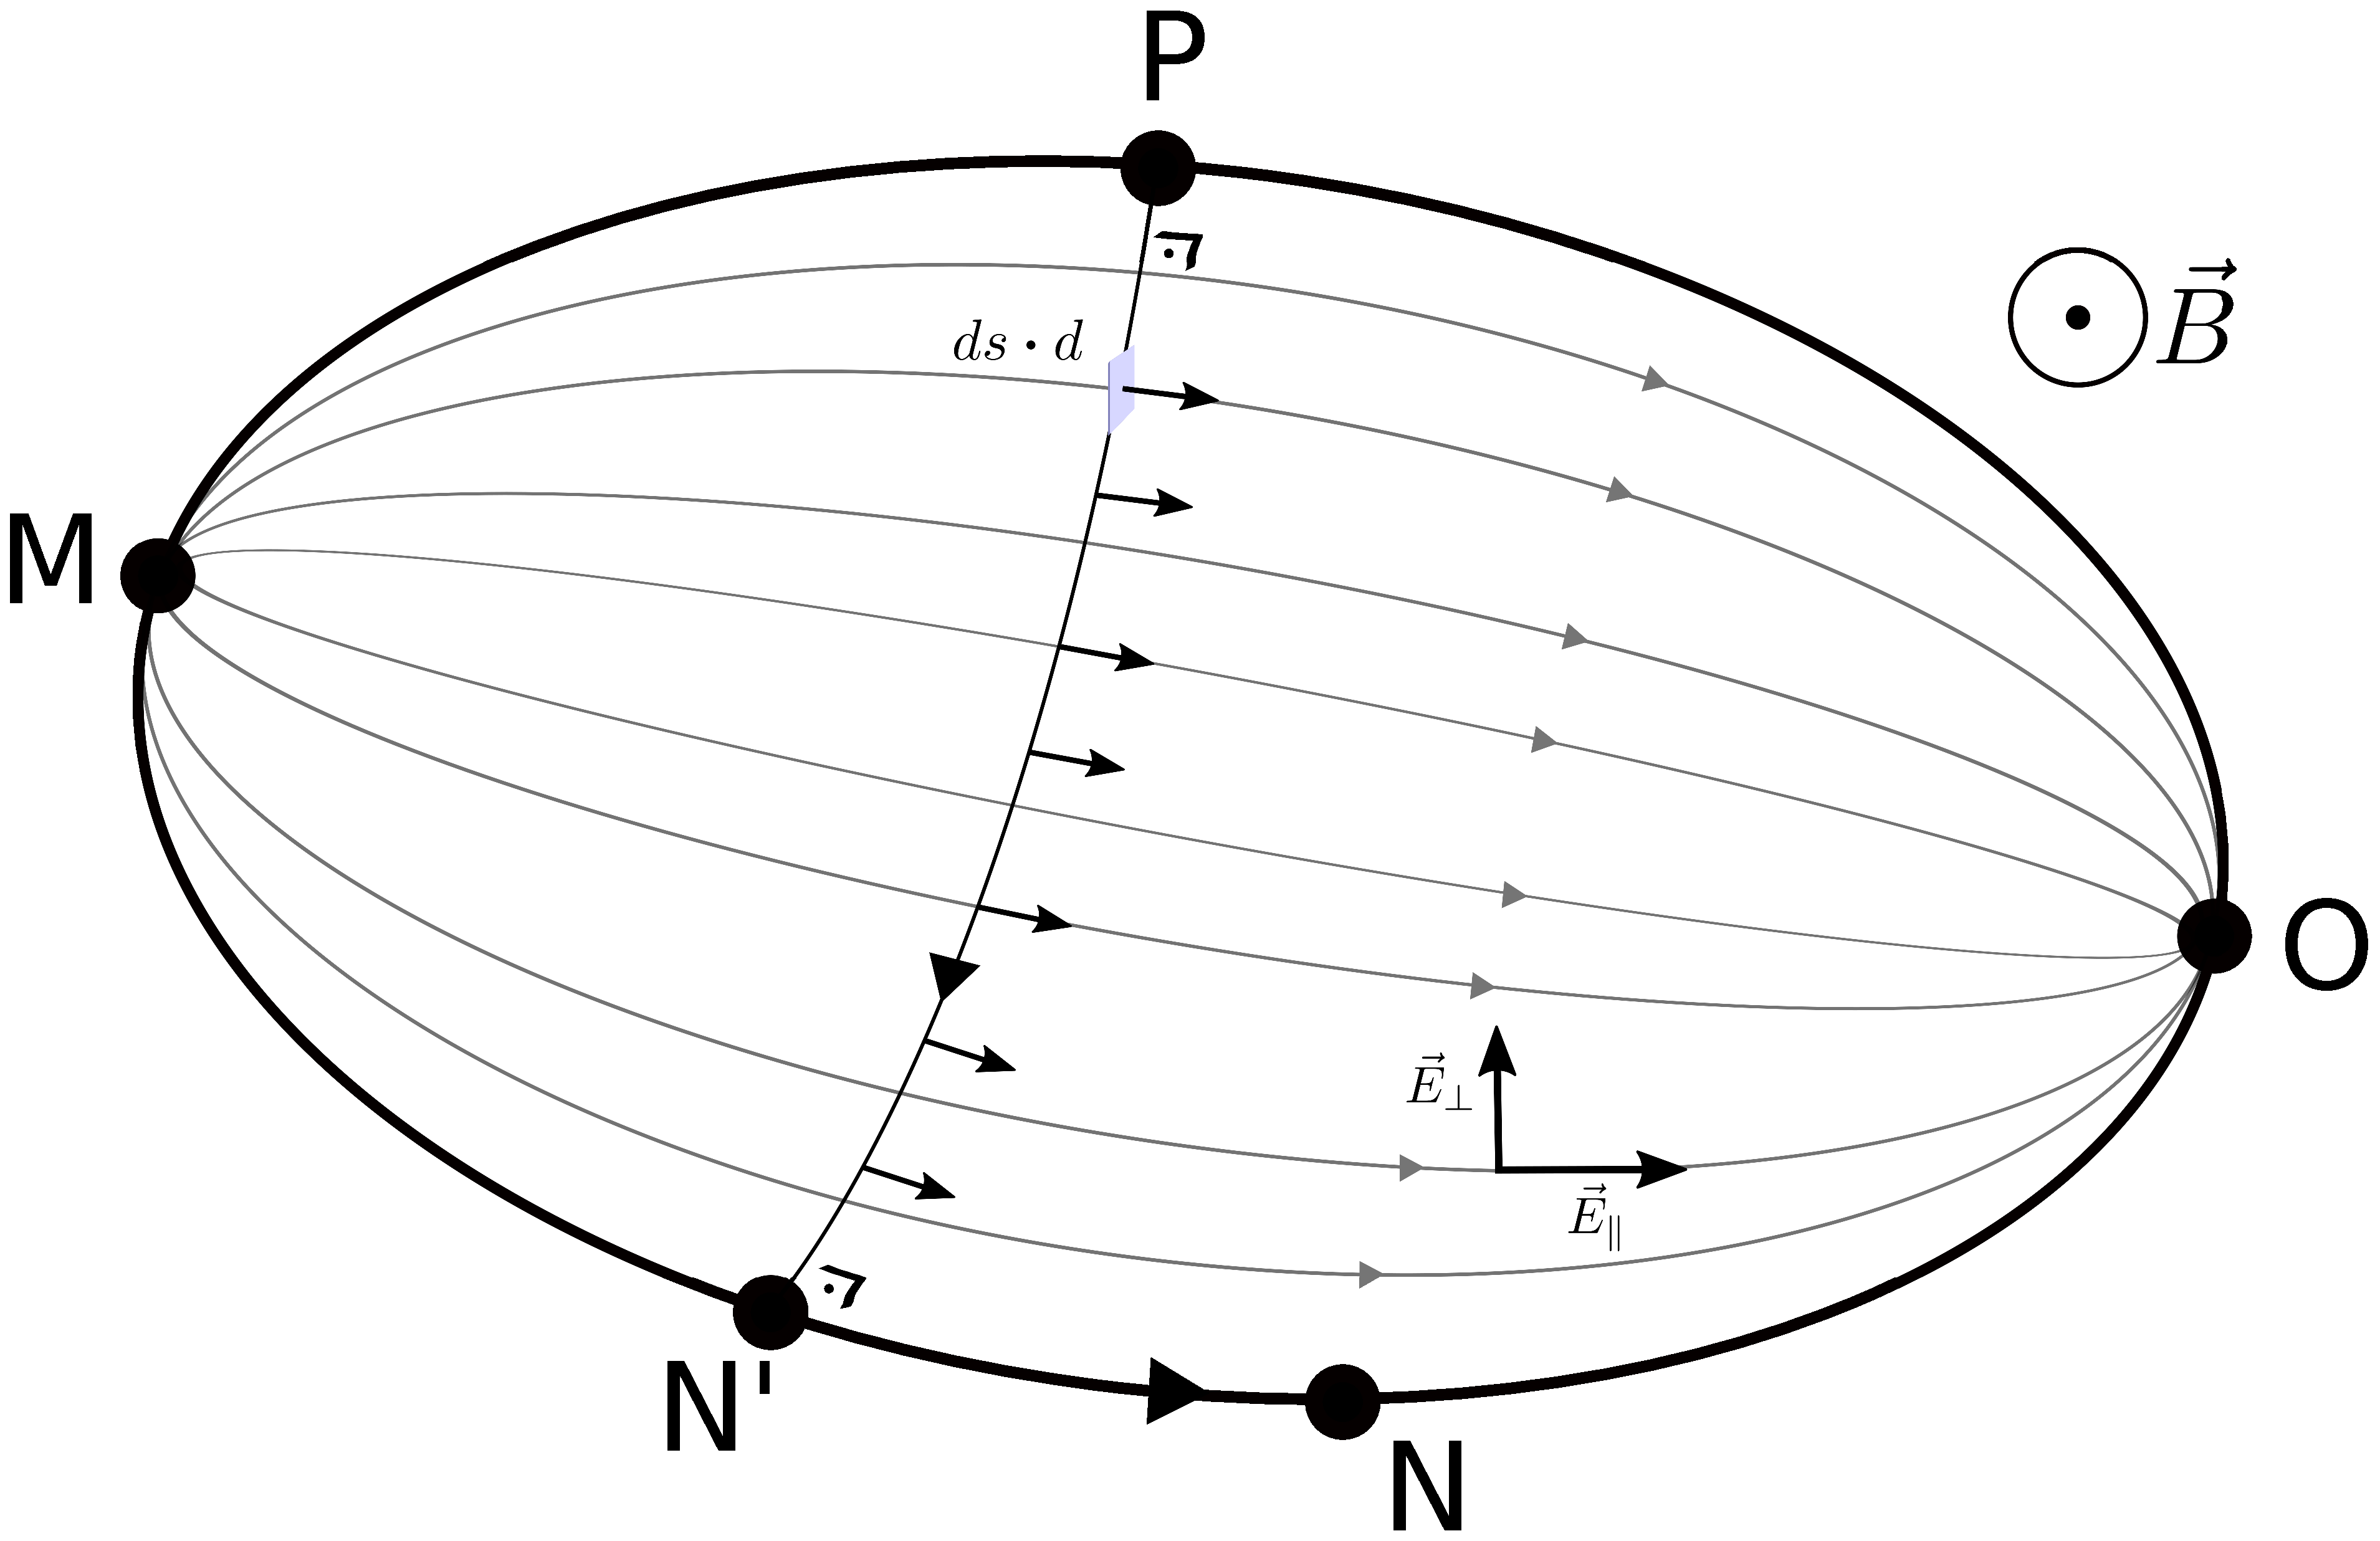
\includegraphics[width=0.9\textwidth]{Drawing.eps}
\caption{Schematic drawing of a semiconductor with four contacts (P, M, N, O). There is a circulating current from M to O, and an external magnetic field perpendicular to the sample pointing upwards. N' is not a physical contact but a reference point to compute the integral explained in the text.}
\label{fig:sample}
\end{figure}

Let us see how we can use this simple model to obtain an expression that relates the voltages that can be measured experimentally and the carrier density $p$.

We begin by considering the sample drawn in Figure \ref{fig:sample}. A current goes from point M to point O and there is a magnetic field $\vec{B}$ perpendicular to the sample. We can write the electric field $\vec{E}$ at each point in terms of a parallel and a perpendicular component with respect to $\vec{j}$:

\begin{equation}\label{eq:E_field}
\vec{E}=\frac{1}{\mu}\vec{v}_d-\vec{v}\times\vec{B}=\frac{1}{ep\mu}\vec{j}-\frac{1}{ep}\left(\vec{j}\times\vec{B}\right)\equiv\vec{E}_\parallel + \vec{E}_\perp
\end{equation}

The potential difference $U_\text{PN}$ can be computed integrating the electric field from P to N. In order to calculate the integral we can exploit the fact that the electric field is a conservative vector field, and thus the line integral is path independent. In particular, we will take the path P to N' and N' to N shown in Figure \ref{fig:sample}.

\begin{equation}\label{eq:U_PN}
U_\text{PN}=\int_P^N\vec{E}\cdot d\vec{s}=\int_P^{N'}\vec{E}_\perp\cdot d\vec{s}+\underbrace{\int_{N'}^N\vec{E}_\parallel\cdot d\vec{s}}_{U_\text{Off}}
\end{equation}

We have called the second term in \eqref{eq:U_PN} \emph{offset voltage} $U_\text{off}$. This terms takes into account that the sample does not have a rectangularly shape (a so-called «Hall bar») and experimentally can be measured by switching off the magnetic field.

The first integral can be evaluated taking into account that the magnetic field is orthogonal to the sample's surface, i.e. $(\vec{j}\times\vec{B})\vdot d\vec{s}=|\vec{j}\times\vec{B}|ds=jB\,ds$. Hence, we obtain:

\begin{equation}
\int_P^{N'}\vec{E}_\perp\cdot d\vec{s}=-\frac{B}{ep}\int_P^{N'}j\, ds=-\frac{B}{ep}\int_P^{N'}\frac{1}{d}\frac{dI}{\cancel{ds}}\, \cancel{ds}=-\frac{B}{epd}\underbrace{\int_P^{N'} dI}_I=-\frac{BI}{epd}
\end{equation}

Defining the Hall coefficient $R_H\equiv\dfrac{1}{ep}$, we get the relation that will allow us to measure the carrier density:
\begin{equation}\label{eq:Hall_voltage}
U_\text{PN}-U_\text{off}=U_\text{Hall}=-R_H\frac{BI}{d}\,,
\end{equation}
when $B$ and $I$ are fixed and the sample's thickness $d$ is known.


After obtaining a formal expression relating the Hall coefficient, and thus the carrier density $p$, with two voltages that can be measured experimentally on a sample not necessary rectangularly shaped, we now continue explaining a method to measure the resistivity.

In 1958, Van der Pauw \cite{vdP} proved that if a voltage is applied by putting sufficiently small contacts at the border of a sample, which is homogeneous in thickness ($d$) and has no isolated holes, then the following formula holds:

\begin{equation}
\exp\left(-\pi R_\text{AB,CD}\,\frac{d}{\rho}\right)+\exp\left(-\pi R_\text{BC,DA}\,\frac{d}{\rho}\right)=1\,,
\end{equation}
where $\rho$ is the resistivity, and the resistance $R_{AB,CD}$ is defined as the ratio between the voltage measured between the contact points C and D and the current applied between the points A and B. Analogously, $R_\text{BC,DA}$ is the voltage between D and A over the current circulating from B to C.

As shown in the paper, the resistivity can be obtained according to the following expression:
\begin{equation}
\rho=\frac{\pi d}{\ln(2)}\frac{R_\text{AB,CD}+R_\text{BC,DA}}{2}\,f\!\left(R_\text{AB,CD},R_\text{BC,DA}\right)
\end{equation}
where the function $f$ can be approximated as
\begin{equation}
f \simeq 1-\left(\frac{R_\text{AB,CD}-R_\text{BC,DA}}{R_\text{AB,CD}+R_\text{BC,DA}}\right)^2 \frac{\ln(2)}{2}-\left(\frac{R_\text{AB,CD}-R_\text{BC,DA}}{R_\text{AB,CD}+R_\text{BC,DA}}\right)^4\left(\frac{\ln(2)^2}{4}-\frac{\ln(2)^3}{12}\right)
\end{equation}

Finally, once the Hall coefficient and the resistivity are known, mobility $\mu$ can be computed using the following expression:

\begin{equation}\label{eq:mobility_exp}
\mu=\frac{|R_H|}{\rho}
\end{equation}

\newpage
\section{Materials and methods}

The experimental setup consisted in a liquid nitrogen cryostat DN1710 by Oxford Instruments Ltd. surrounded at the bottom by an electromagnet Bruker Magnet B-E 10 (see Figure \ref{fig:experimental_setup_all}).

Sample was connected to a HP 34401A Digital Multimeter and a Yokogawa 7651 Programmable DC Source. In order to select to which sample contacts they were connected, device shown in Figure \ref{fig:cables} was used.

\begin{figure}[H]
\centering
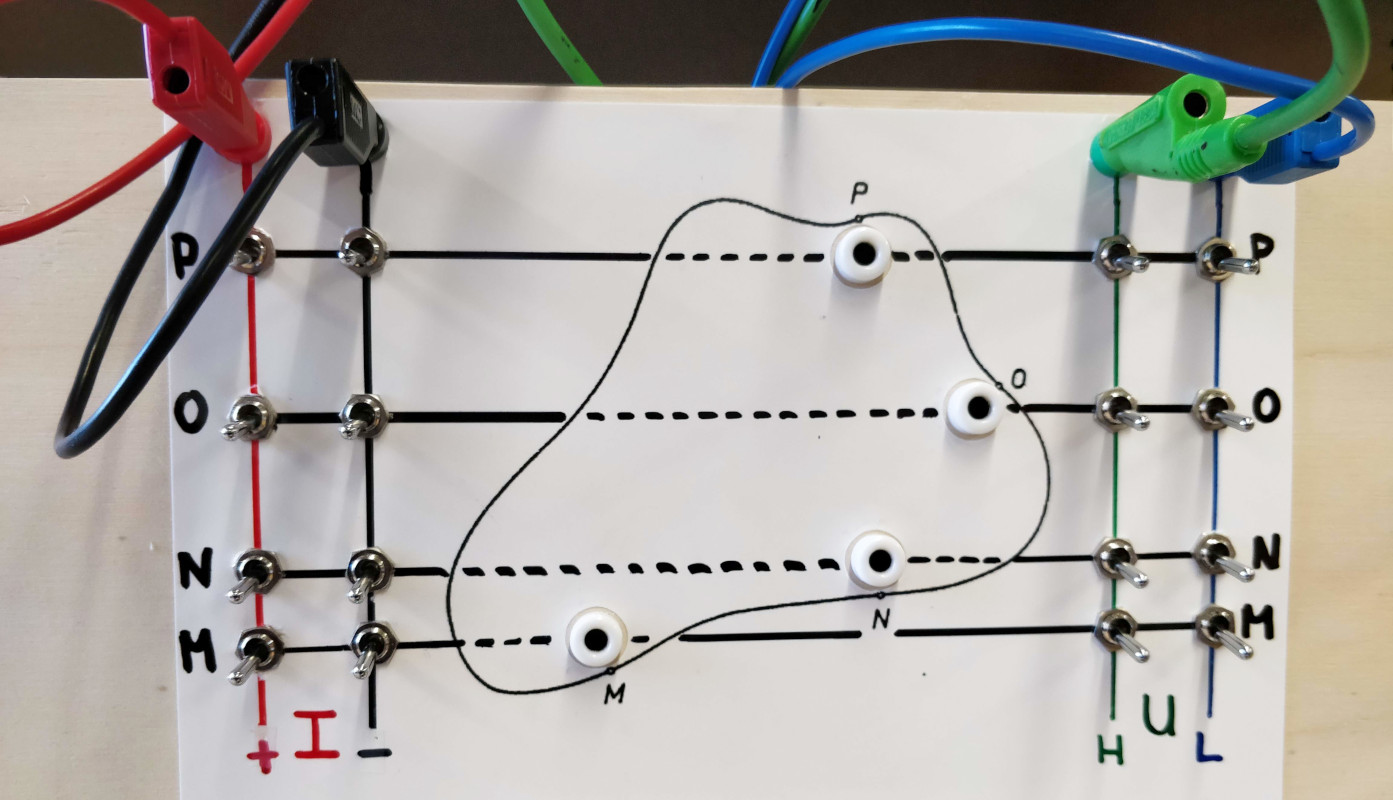
\includegraphics[width=0.6\textwidth]{Experimental_setup_cables}
\caption{Device used to choose where to apply current in the semiconductor sample and where to measure voltage. For example, by turning on switches M and O on the left (current), and switches P and N on the right (voltages), we can measure the transverse voltage $U_t$.}
\label{fig:cables}
\end{figure}

For the characterization of the magnetic field, a calibrated Hall sensor (see Figure \ref{fig:Hall_sensor}) was used connected to the probe tube.

\begin{figure}[H]
\centering
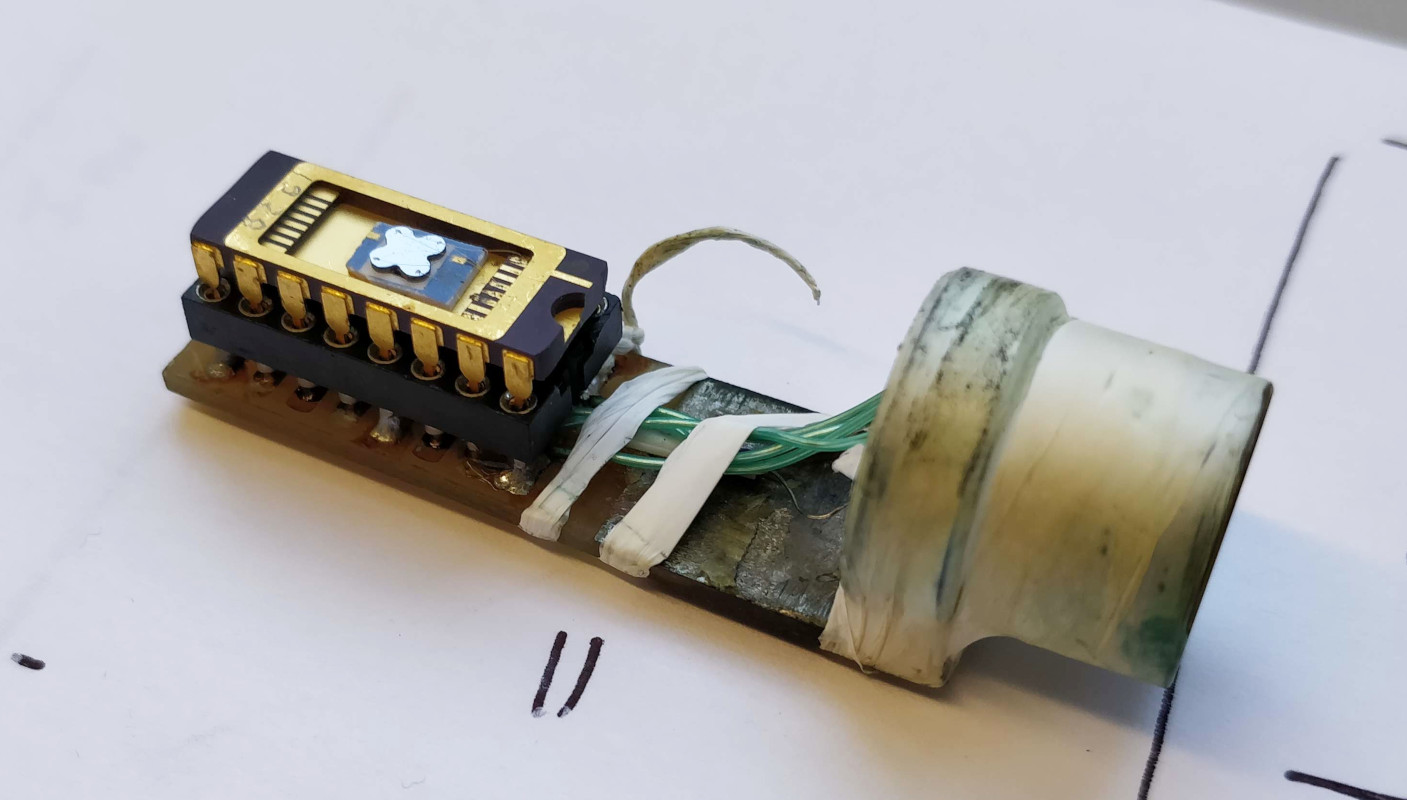
\includegraphics[width=0.5\textwidth]{Hall_sensor}
\caption{Calibrated Hall sensor (\SI{0.1172}{\tesla/\milli\volt} at \SI{10}{\milli\ampere}) used to measure the magnetic field produced by the coils.}
\label{fig:Hall_sensor}
\end{figure}

Finally, determination of the temperature close to the sample was done with a resistor connected to a device that directly show us the temperature in Kelvin (see Figure \ref{fig:temperature_device}). With the same device, we could control a heating mechanism by applying a voltage to a different resistor in the cryostat.

\begin{figure}[H]
\centering
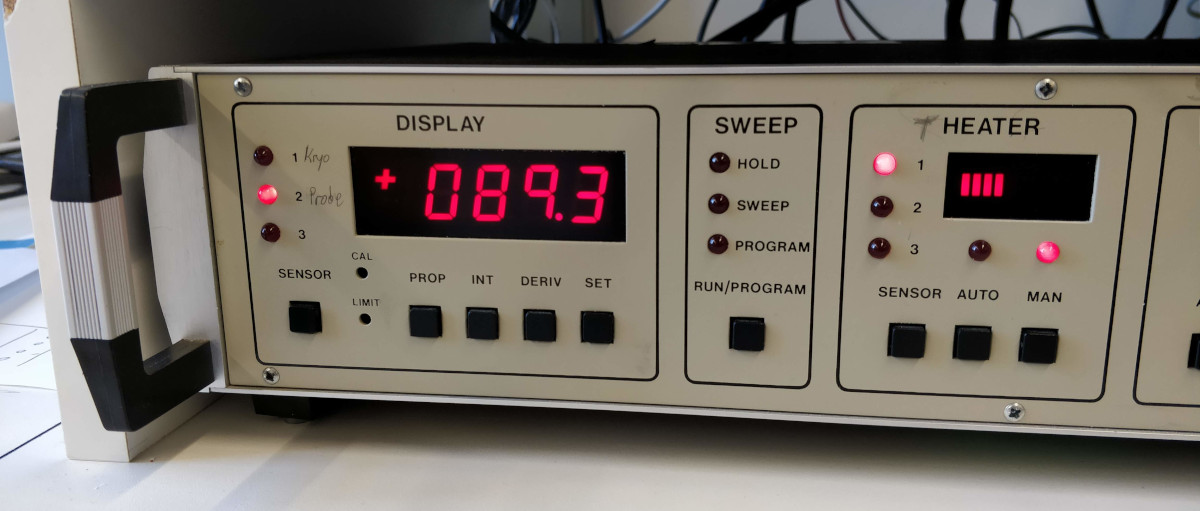
\includegraphics[width=0.5\textwidth]{temperature_device}
\caption{Device showing that temperature close to the sample is \SI{89.3}{\kelvin}. A voltage of \SI{8}{\volt} was being used at that moment to heat the sample after closing the gas exhaust valve.}
\label{fig:temperature_device}
\end{figure}

\begin{figure}[H]
\centering
\begin{subfigure}[b]{0.4\textwidth}
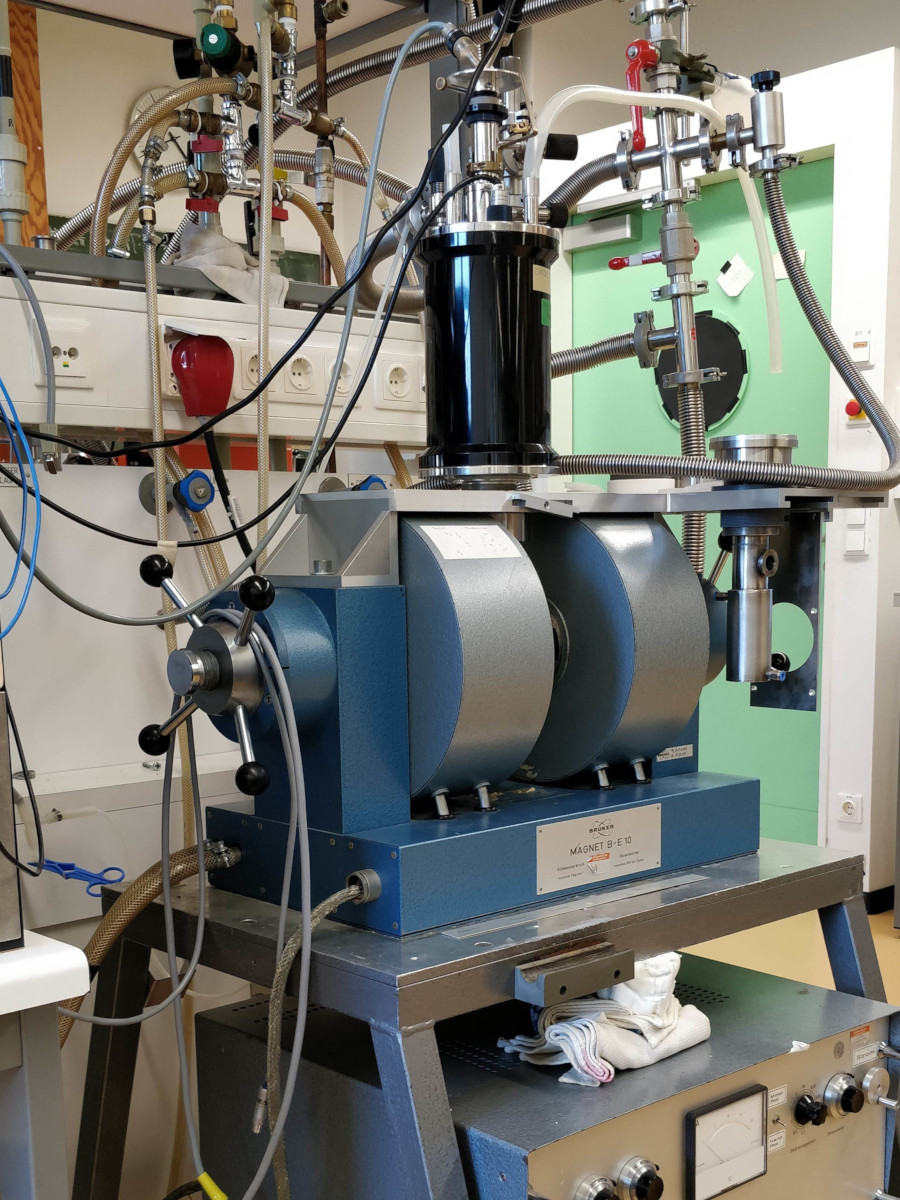
\includegraphics[width=\textwidth]{Experimental_setup}
\caption{}
\label{fig:experimental_setup}
\end{subfigure}
\begin{subfigure}[b]{0.4\textwidth}
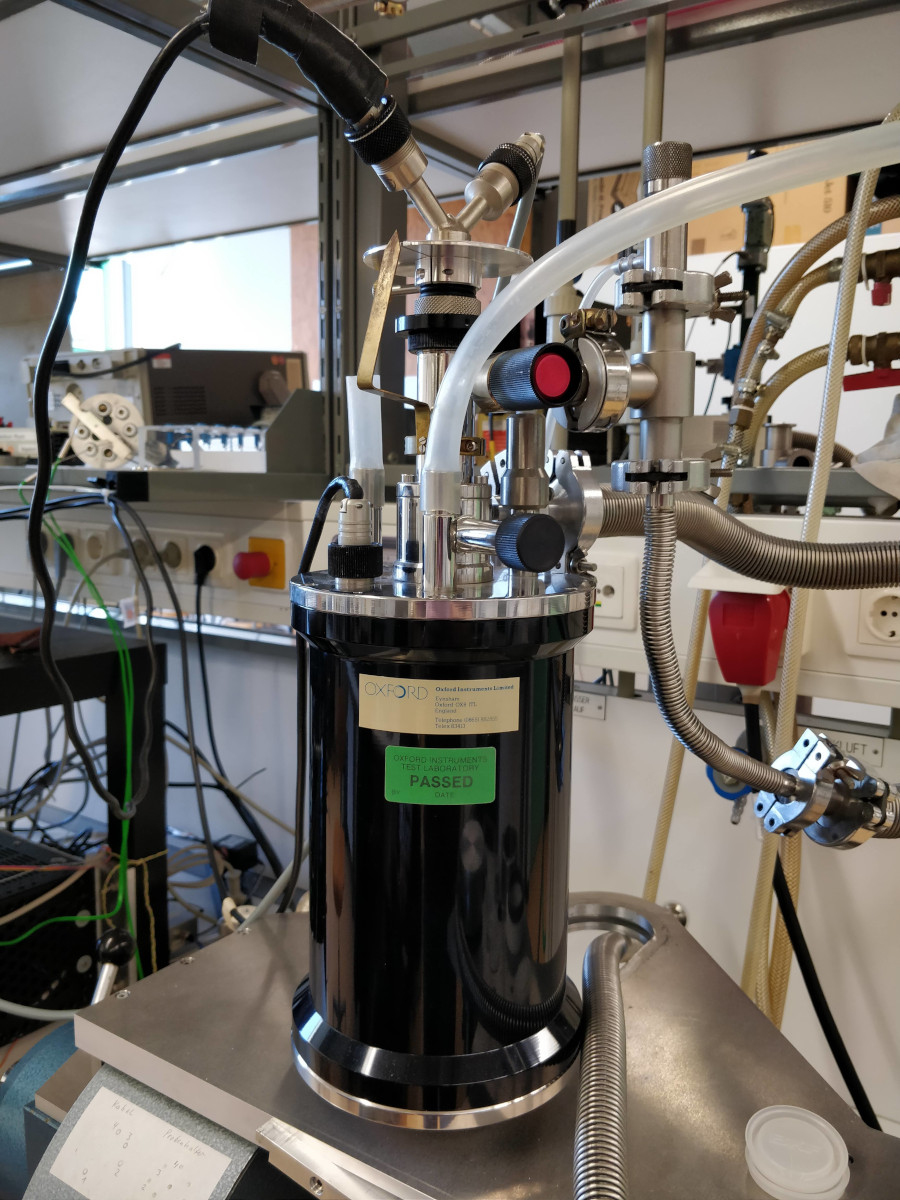
\includegraphics[width=\textwidth]{cryostat}
\caption{}
\label{fig:cryostat}
\end{subfigure}\\\vspace{.2cm}
\begin{subfigure}[b]{0.5\textwidth}
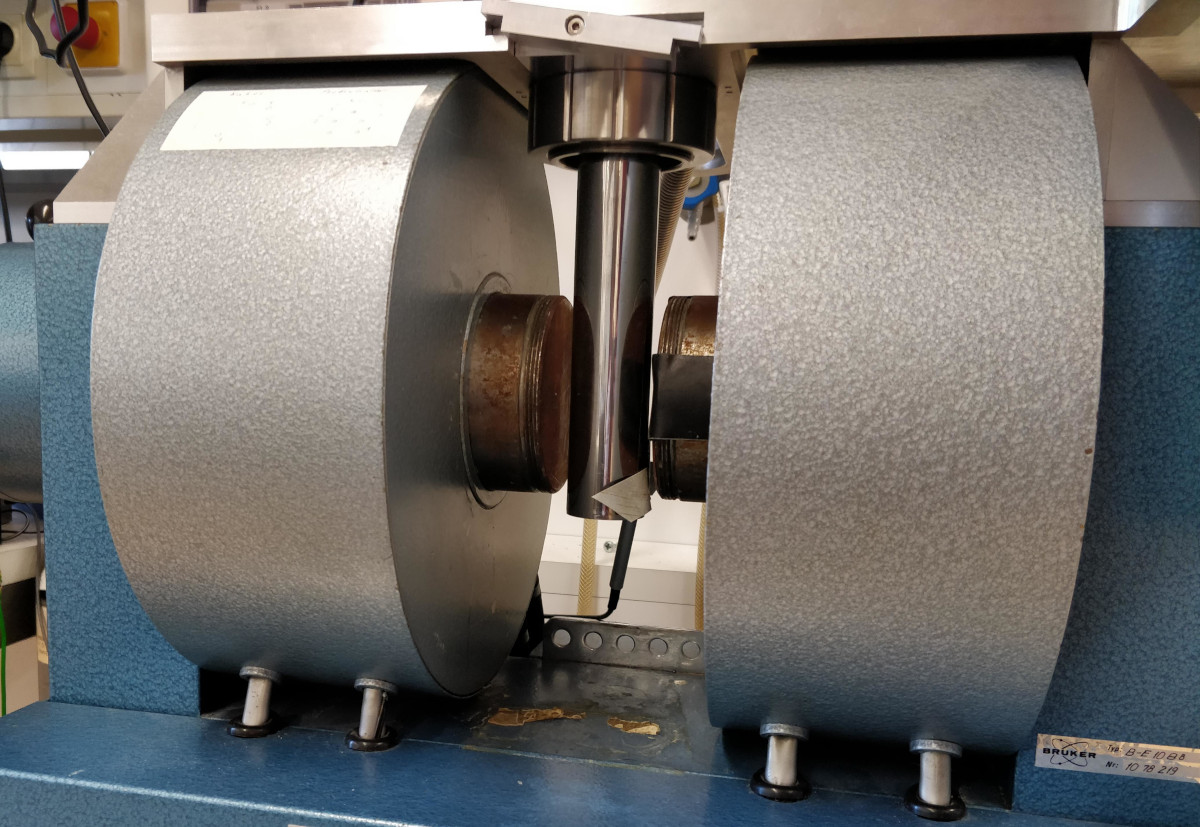
\includegraphics[width=\textwidth]{electromagnet}
\caption{}
\label{fig:electromagnet}
\end{subfigure}
\caption{Experimental setup used for this experiment. In (a) the cryostat with the bottom, where the sample is placed, enclosed by the magnetic coils. In (b) the cryostat in more detail. Transparent tube in the center is connected to a vacuum pump. Left one is the nitrogen entry port. Black valve in the center is the gas exhaust valve. By closing it, temperature starts to rise. Sample is introduced using a probe tube in the sample access port at the top centre. In both (a) and (b) probe tube is already introduced and the cables connected to sample's contacts can be seen, as well as tip to determine the angle between sample and magnetic field. In (c) the electromagnet in detail.}
\label{fig:experimental_setup_all}
\end{figure}

\newpage
\section{Results and discussion}

\subsection{Calibration of the electromagnet}

We determined the dependence of the magnetic field strength $B$ on the current $I_B$ through the magnetic coils using a calibrated Hall sensor (see Figure \ref{fig:Hall_sensor}).

We measured the voltage for different currents $I_B$ from \SI{0}{\ampere} to \SI{15}{\ampere} in steps of \SI{1}{\ampere} at room temperature ($\sim\SI{300}{\kelvin}$). In Figure \ref{fig:magnetic_field}, the magnetic field computed using the calibration coefficient (see caption Figure \ref{fig:Hall_sensor}) is plotted against the current $I_B$.

\begin{figure}[H]
\centering
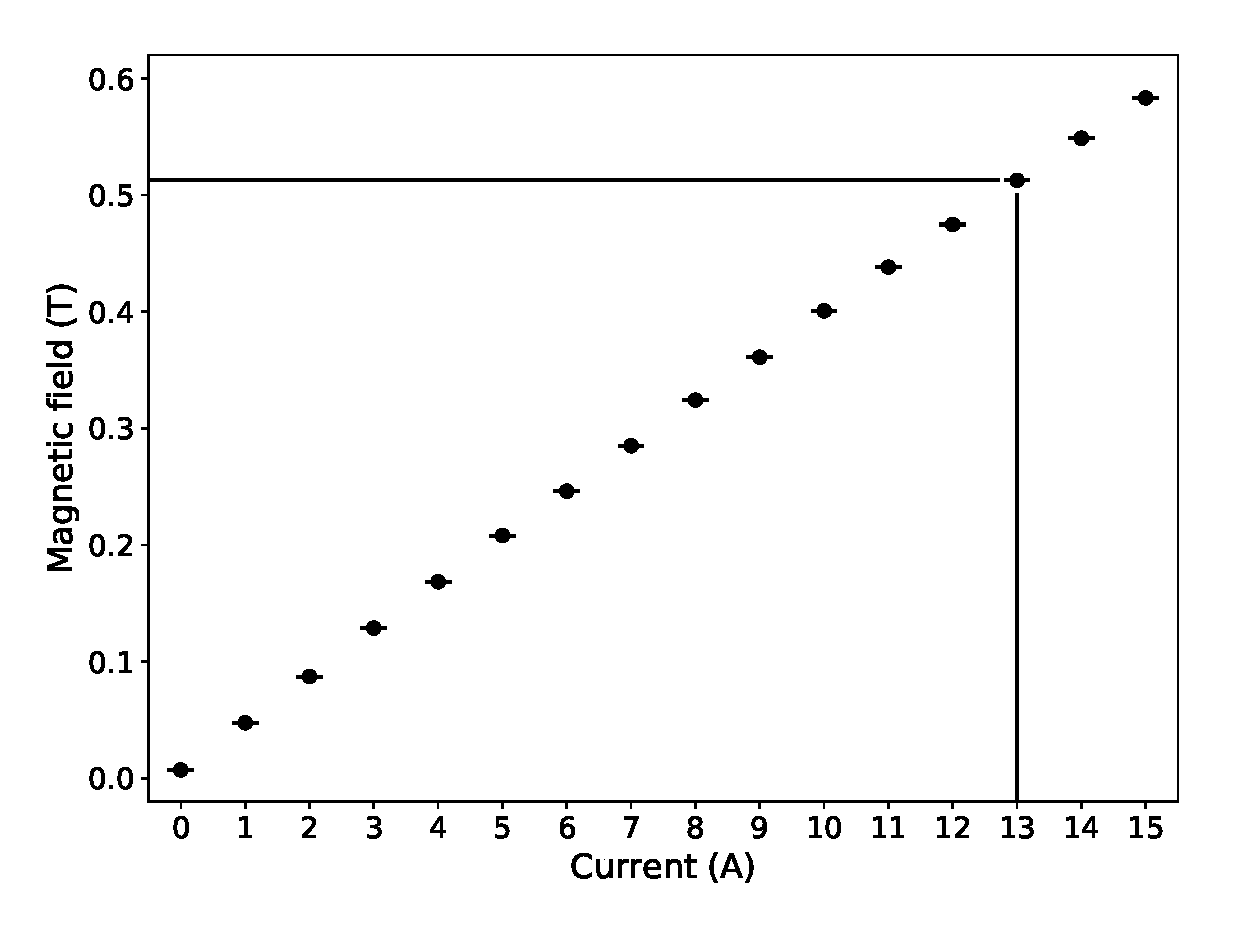
\includegraphics[width=0.6\textwidth]{Magnetic_field_vs_current.eps}
\caption{Magnetic field vs current in the magnetic coils. Solid lines show the current we fixed in the coils for the following measurements, generating a magnetic field of \SI{0.5126}{\tesla}.}
\label{fig:magnetic_field}
\end{figure}

\subsection{Checking ohmic behaviour}

The junction between conductors should have a linear current-voltage curve. We checked this by measuring the voltage between two points for currents from \SI{0}{\micro\ampere} to \SI{150}{\micro\ampere} in steps of \SI{10}{\micro\ampere} also at room temperature. In Figure \ref{fig:ohmic_check}, the linear behaviour is clearly showed.

\begin{figure}[H]
\centering
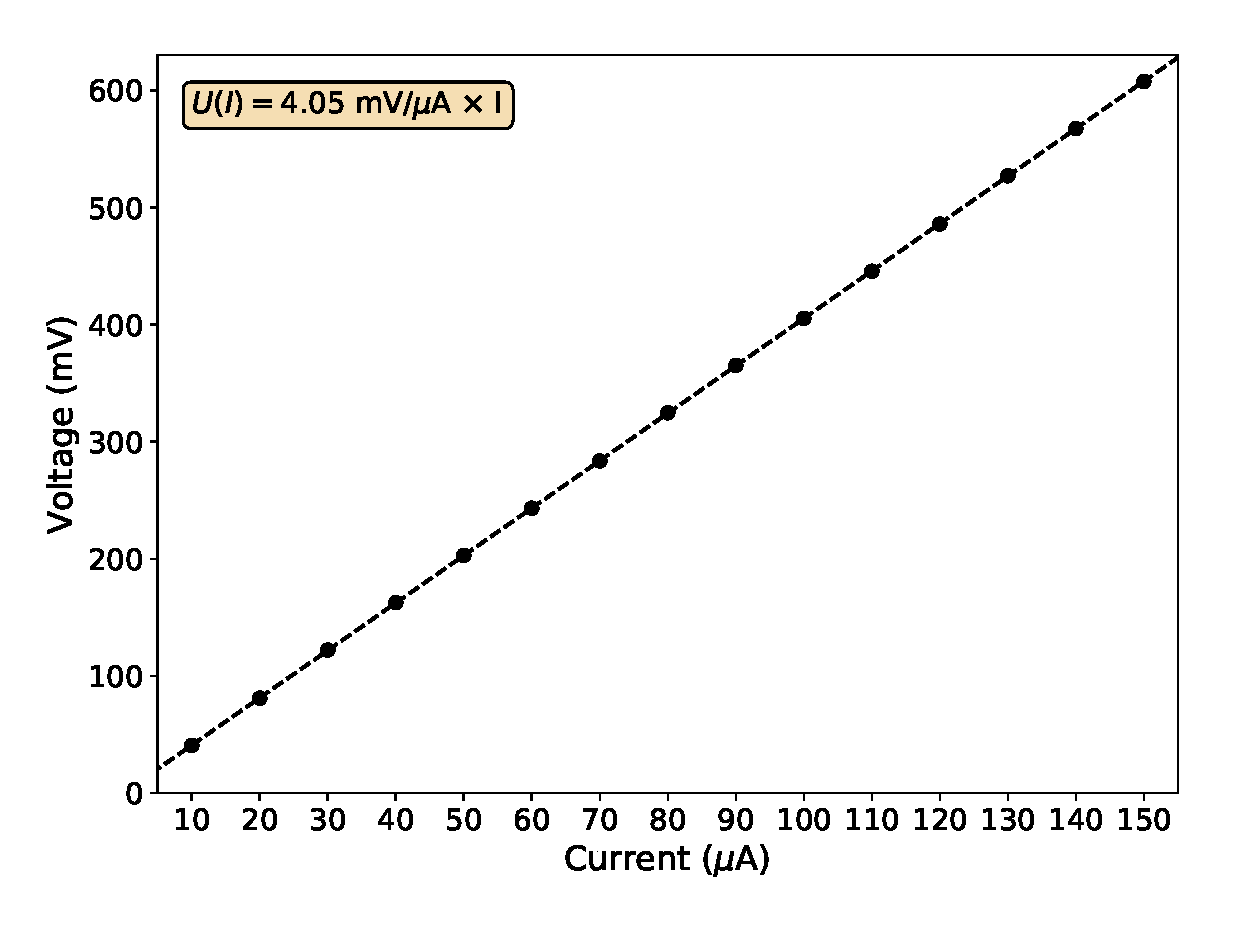
\includegraphics[width=0.6\textwidth]{Voltage_vs_current_ohmic_test.eps}
\caption{Measured voltage vs applied current between two sample contacts. The dashed line is a linear fit of the experimental data with slope \SI{4.05}{\milli\volt/\milli\ampere}.}
\label{fig:ohmic_check}
\end{figure}

\subsection{Orientation of the sample}

In order to align the sample perpendicular to the magnetic field generated by the coils, we measured the transverse voltage $U_t$, i.e. the Hall voltage plus the offset voltage, with a fixed magnetic field $B=\SI{0.5126}{\tesla}$ and a current $I=\SI{100}{\micro\ampere}$ for different angles between the magnetic field and the surface normal of the sample from \ang{-90} to \ang{90} in steps of \ang{10}.

\begin{figure}[H]
\centering
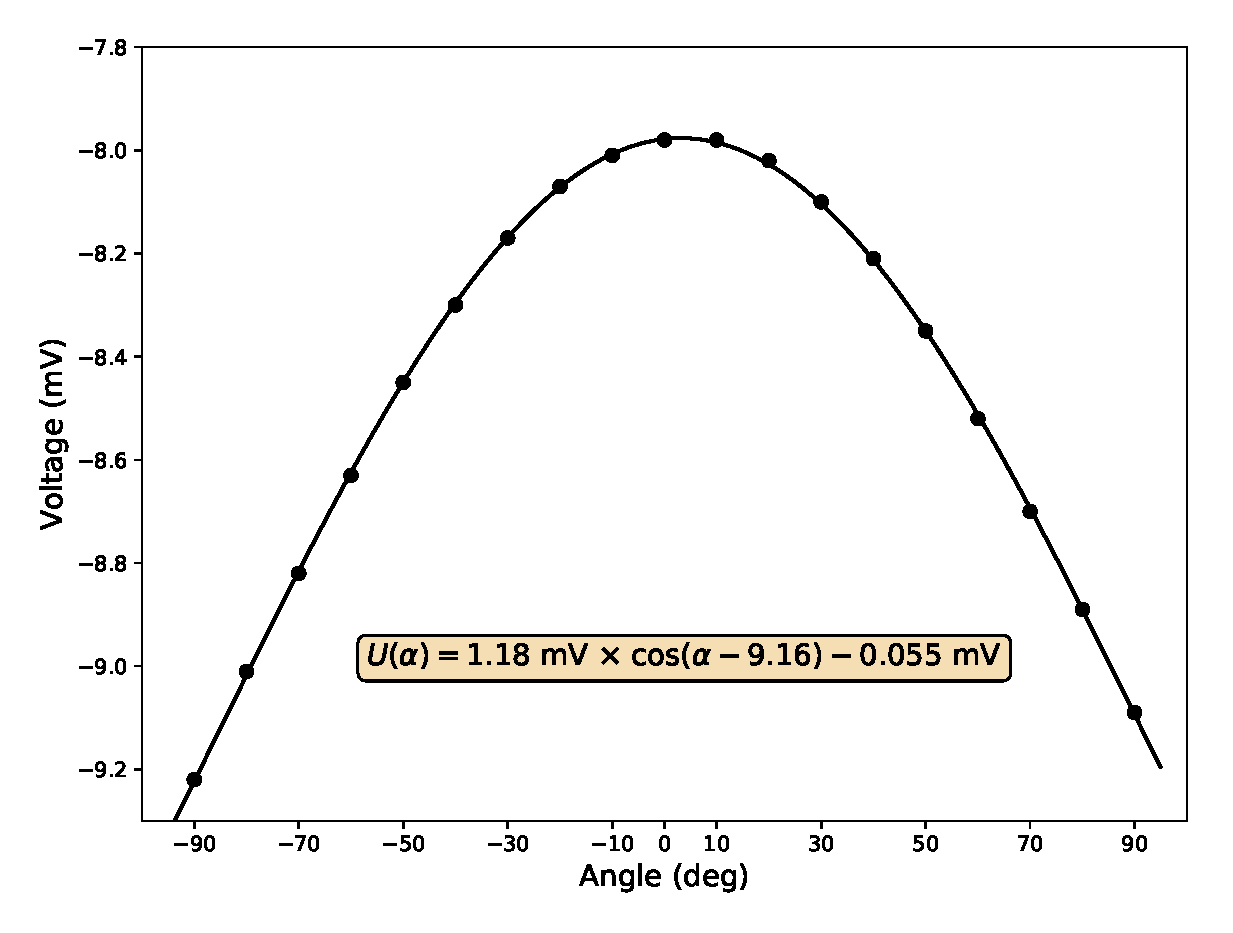
\includegraphics[width=0.7\textwidth]{Voltage_vs_angle.eps}
\caption{Transverse voltage vs orientation angle of the sample with respect to the applied magnetic field. Dash line is a fit using the function $U_t(\alpha)=U_0\cos(\alpha+\phi) + U_\text{off}$. Values obtained for the fitting parameters are shown in the plot box.}
\label{fig:orientation}
\end{figure}

\subsection{Determination of $p$ and $\mu$}

After the calibration measurements, we cooled down the sample to about \SI{80}{\kelvin} using liquid nitrogen. At a temperature of \SI{82}{\kelvin} we started to do the following measurements every \SI{5}{\kelvin} while warming up the sample applying a voltage to a resistor in the cryostat. Temperature was measured by a different resistor close to the sample.
\begin{itemize}
\item Offset voltage $U_\text{off}$, i.e. the potential difference between contacts P and N while applying a current of \SI{100}{\micro\ampere} between contacts M and O and without magnetic field (see Figure \ref{fig:cables}).
\item Transverse voltage $U_t$ between contacts P and N, i.e. the sum of Hall voltage and the offset voltage, while applying same current of \SI{100}{\micro\ampere} between M and O and with a magnetic field of \SI{0.5126}{\tesla}.
\item The potential difference $U_\text{OP}$ between contacts O and P while applying a current of \SI{100}{\micro\ampere} between contacts M and N and with the same magnetic field as before.
\item The potential difference $U_\text{PM}$ between contacts P and M while applying the same current between contacts N and O and under the same magnetic field.
\end{itemize}

First two measurements are used to compute the Hall coefficient $R_H$ and the carrier concentration $p$ of our p-doped semiconductor. The other two are necessary to obtain the resistivity $\rho$ using the van der Pauw method \cite{vdP}. Once $R_H$ and $\rho$ are known, it is also possible to compute the Hall mobility $\mu_H$.

We were able to measure these four values from \SI{82}{\kelvin} to \SI{200}{\kelvin}, but heating process was too slow to reach \SI{300}{\kelvin} so we were given measurements from other group. We combined theirs with ours to get the full range of temperatures (see Appendix \ref{app:dataset}).

We can obtain Hall coefficient from equation \eqref{eq:Hall_voltage} but we have to be careful with units. When Hall voltage is expressed in \si{\milli\volt}, magnetic field in \si{\tesla} and current in \si{\ampere}, we have to divide by 10 as shown next in order to obtain the Hall coefficient in the desired units of \si{\centi\meter^3/\coulomb}.

\begin{equation*}
R_H=\frac{d}{BI}U_\text{Hall}\,[=]\,\frac{\si{\centi\meter}}{\si{\tesla\ampere}}\si{\milli\volt}\,[=]\,\frac{\si{\centi\meter}}{\si{\ampere}}\frac{\si{\meter^2}}{\si{\volt\second}}\si{\milli\volt}\,[=]\,\frac{10^4}{10^3}\frac{\si{\centi\meter^3}}{\si{\milli\volt\coulomb}}\si{\milli\volt}\,[=]\,10\,\frac{\si{\centi\meter^3}}{\si{\coulomb}}
\end{equation*}

\begin{figure}[H]
\centering
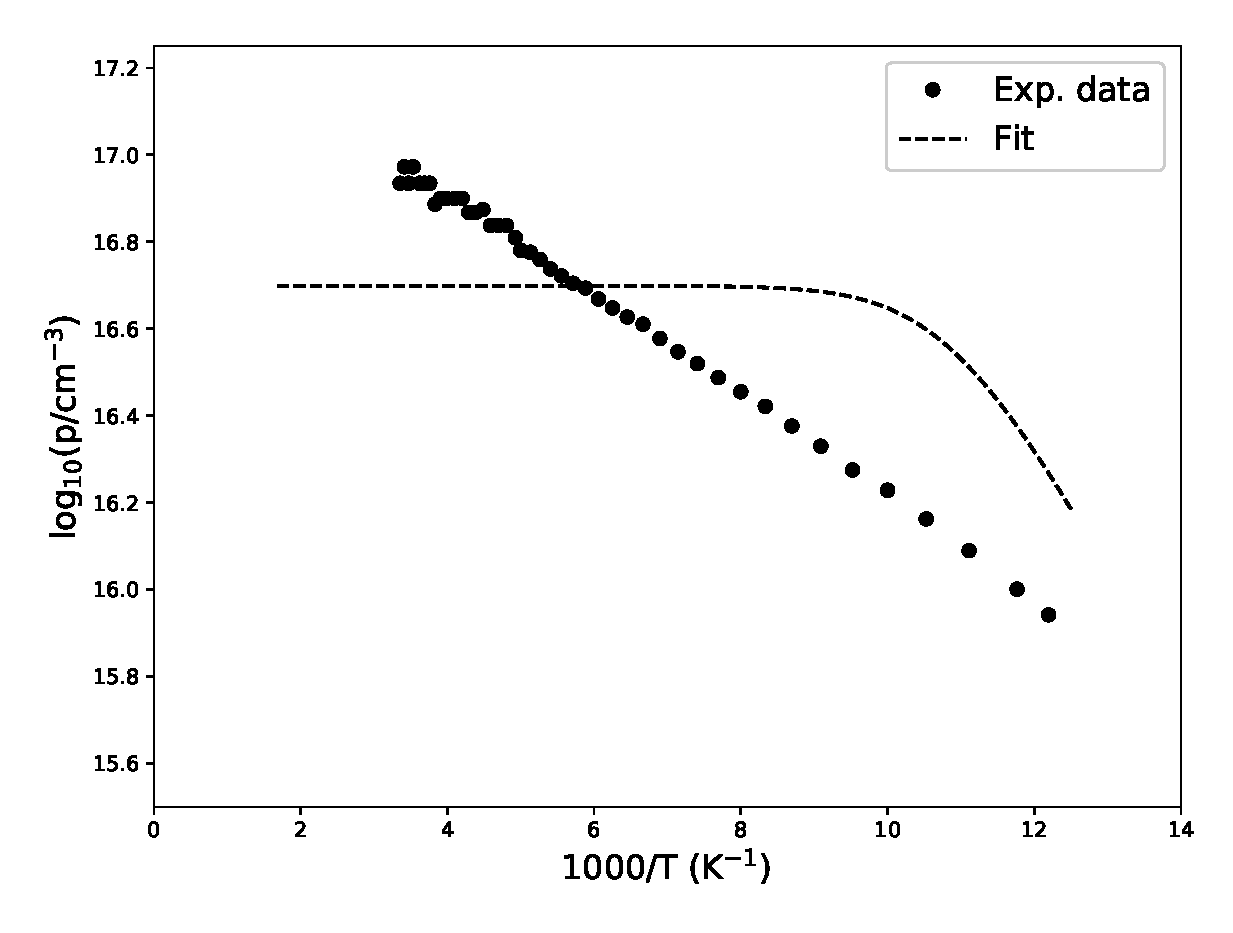
\includegraphics[width=.7\textwidth]{carrier_density.eps}
\caption{Experimentally obtained carrier density $p$ for different temperatures. Dots are experimental values, dashed line is a fit using equation \eqref{eq:p_final} to obtain $N_A$ and $E_a$, and dashdotted line is equation \eqref{eq:p_final_approx} plotted using obtained parameters from previous fit for this range of temperatures.}
\label{fig:carrier_density}
\end{figure}

\begin{figure}[H]
\centering
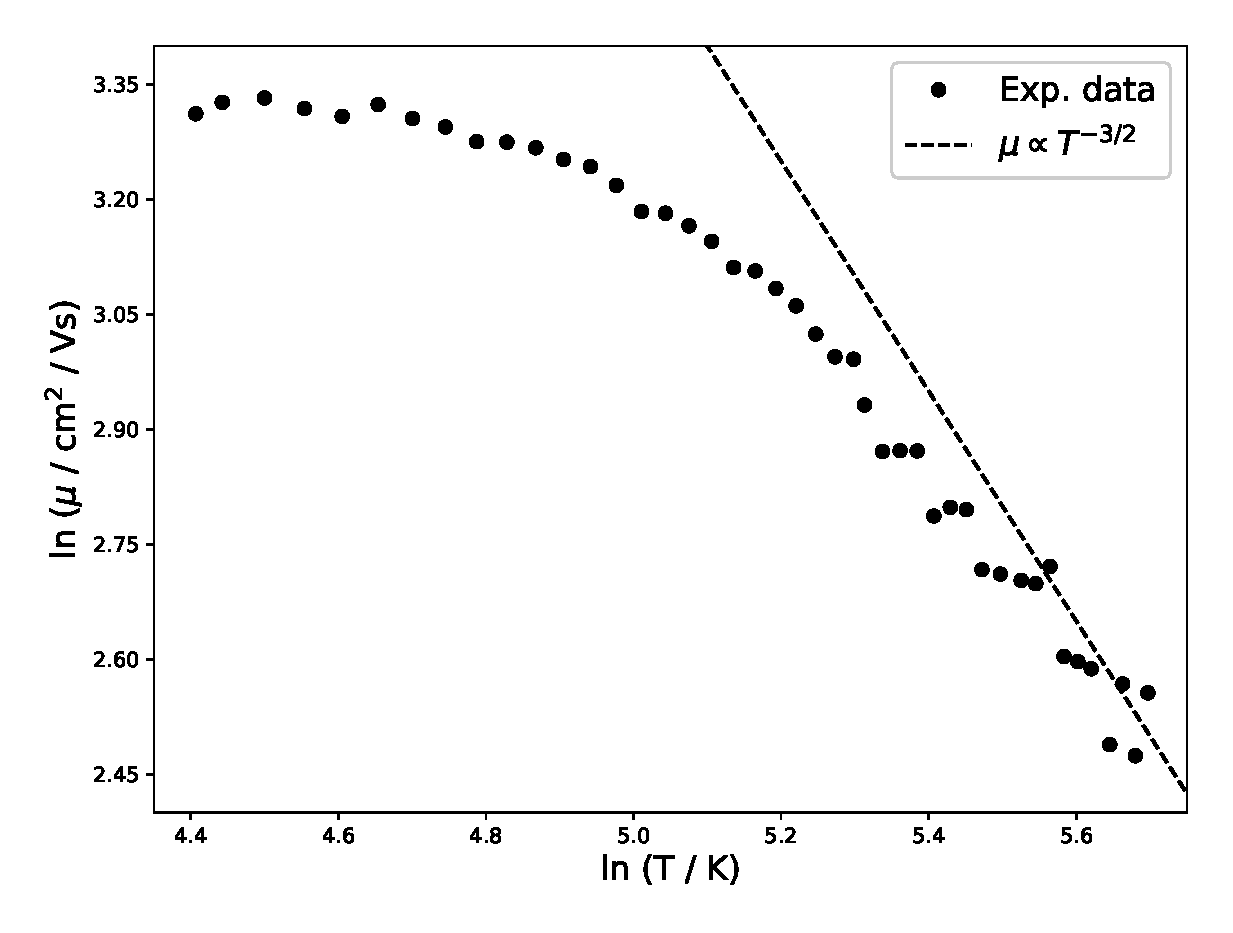
\includegraphics[width=.7\textwidth]{Hall_mobility.eps}
\caption{Experimentally obtained mobility $\mu$ for different temperatures.}
\label{fig:hall_mobility}
\end{figure}

%\section{Conclusions}

\nocite{*}
\vfill
\bibliographystyle{unsrt}
\bibliography{references}

\newpage
\begin{appendices}
\section{Joining measurements}\label{app:dataset}
Due to a problem with the heating mechanism in the cryostat, we could only do measurements from \SI{82}{\kelvin} to \SI{200}{\kelvin}. The complete raw data from a different group was given to us so we would have measurements in the range from \SI{80}{\kelvin} to \SI{300}{\kelvin}. In this appendix we compare our measurements at low temperatures with theirs, and we showed how he generate a combined dataset.

In Figure \ref{fig:comparison_datasets} we summarize the comparison of both datasets. There is a good enough agreement between them so we decided to join them together and use our measurements at low temperatures and theirs from \SI{200}{\kelvin} to \SI{300}{\kelvin}. The noticeable deviation at low temperatures may be due to the fact that they aligned the sample at a slightly different angle with the magnetic field. This angle was not included in the their dataset but deviation is negligible at higher temperatures.

\begin{figure}[H]
\centering
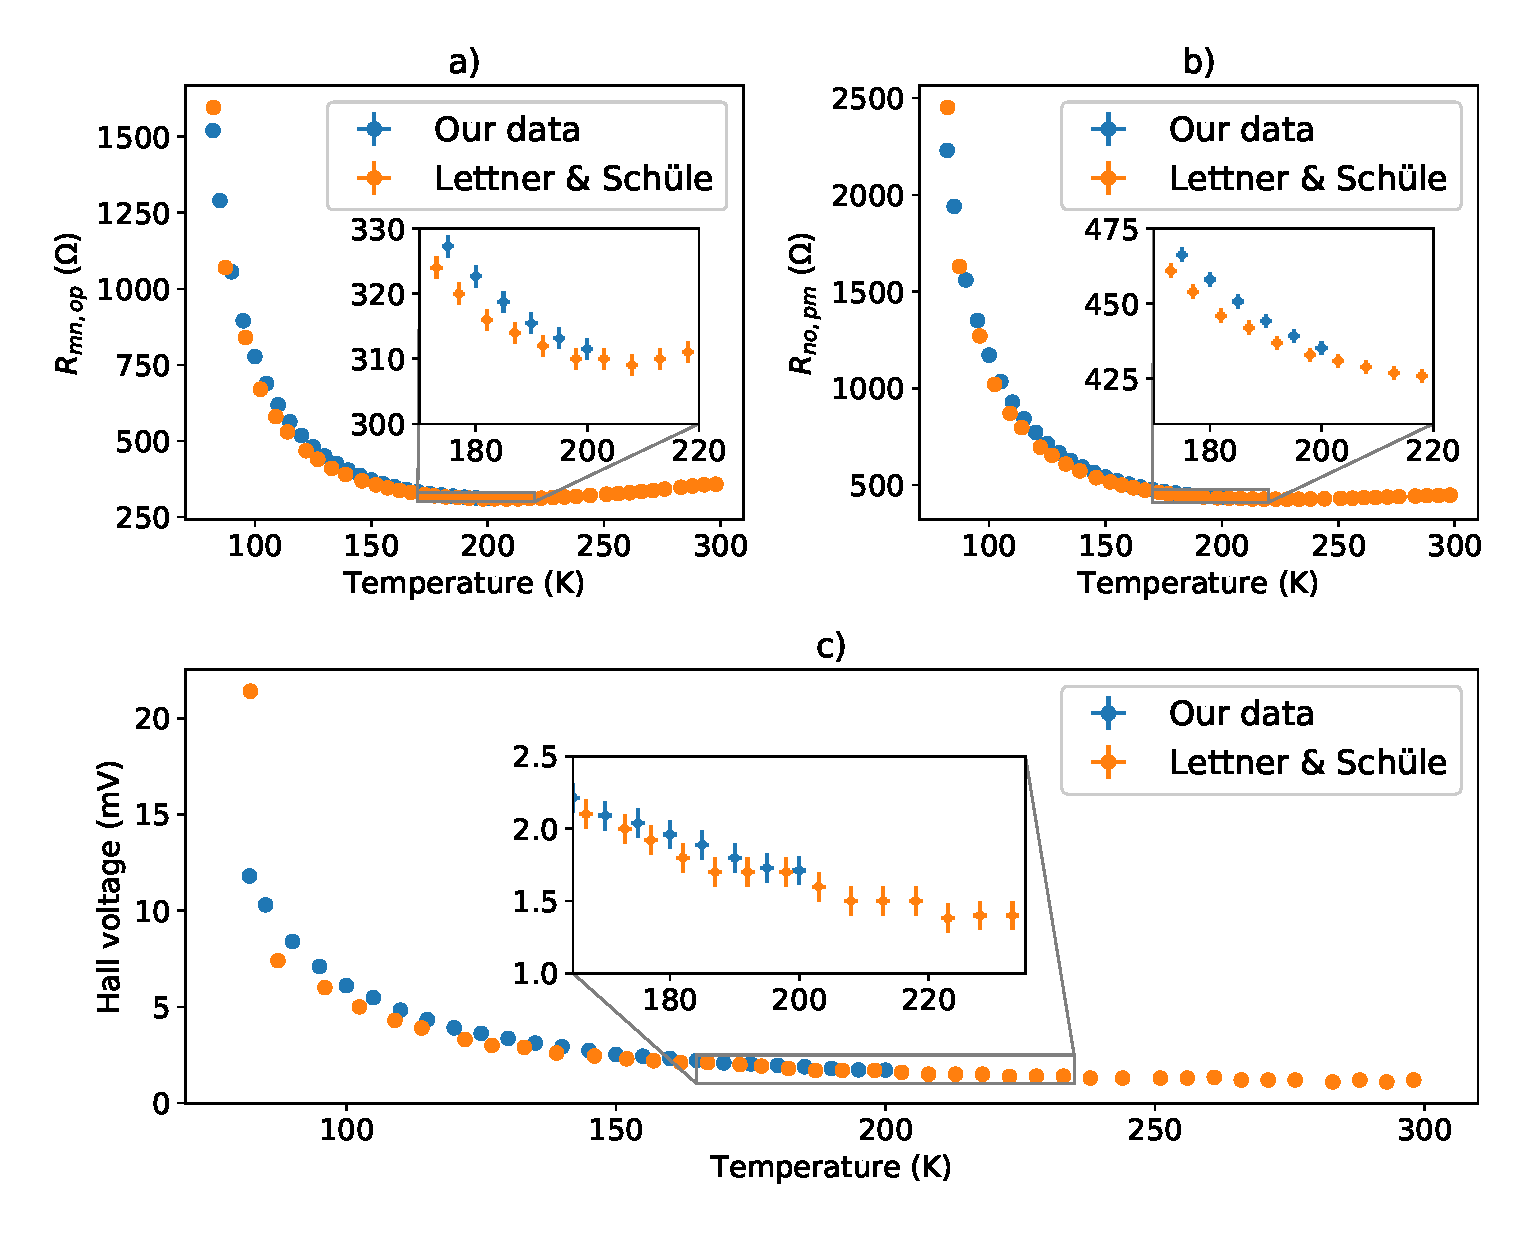
\includegraphics[width=\textwidth]{comparison_datasets.eps}
\caption{In a) and b) the two resistances computed from the measured voltages and in c) the Hall voltage are plotted against temperature. Blue dots represent our measurements and orage dots the values obtained by the other group. Zoomed areas are drawn around $T=\SI{200}{\kelvin}$ to better show the union between our measurements and theirs for our last recorded temperature.}
\label{fig:comparison_datasets}
\end{figure}

Final dataset consists of 25 temperatures from our dataset and 19 from theirs and it is shown in Figure \ref{fig:final_dataset}. All the plots in the report are obtained using this dataset.

\begin{figure}[H]
\centering
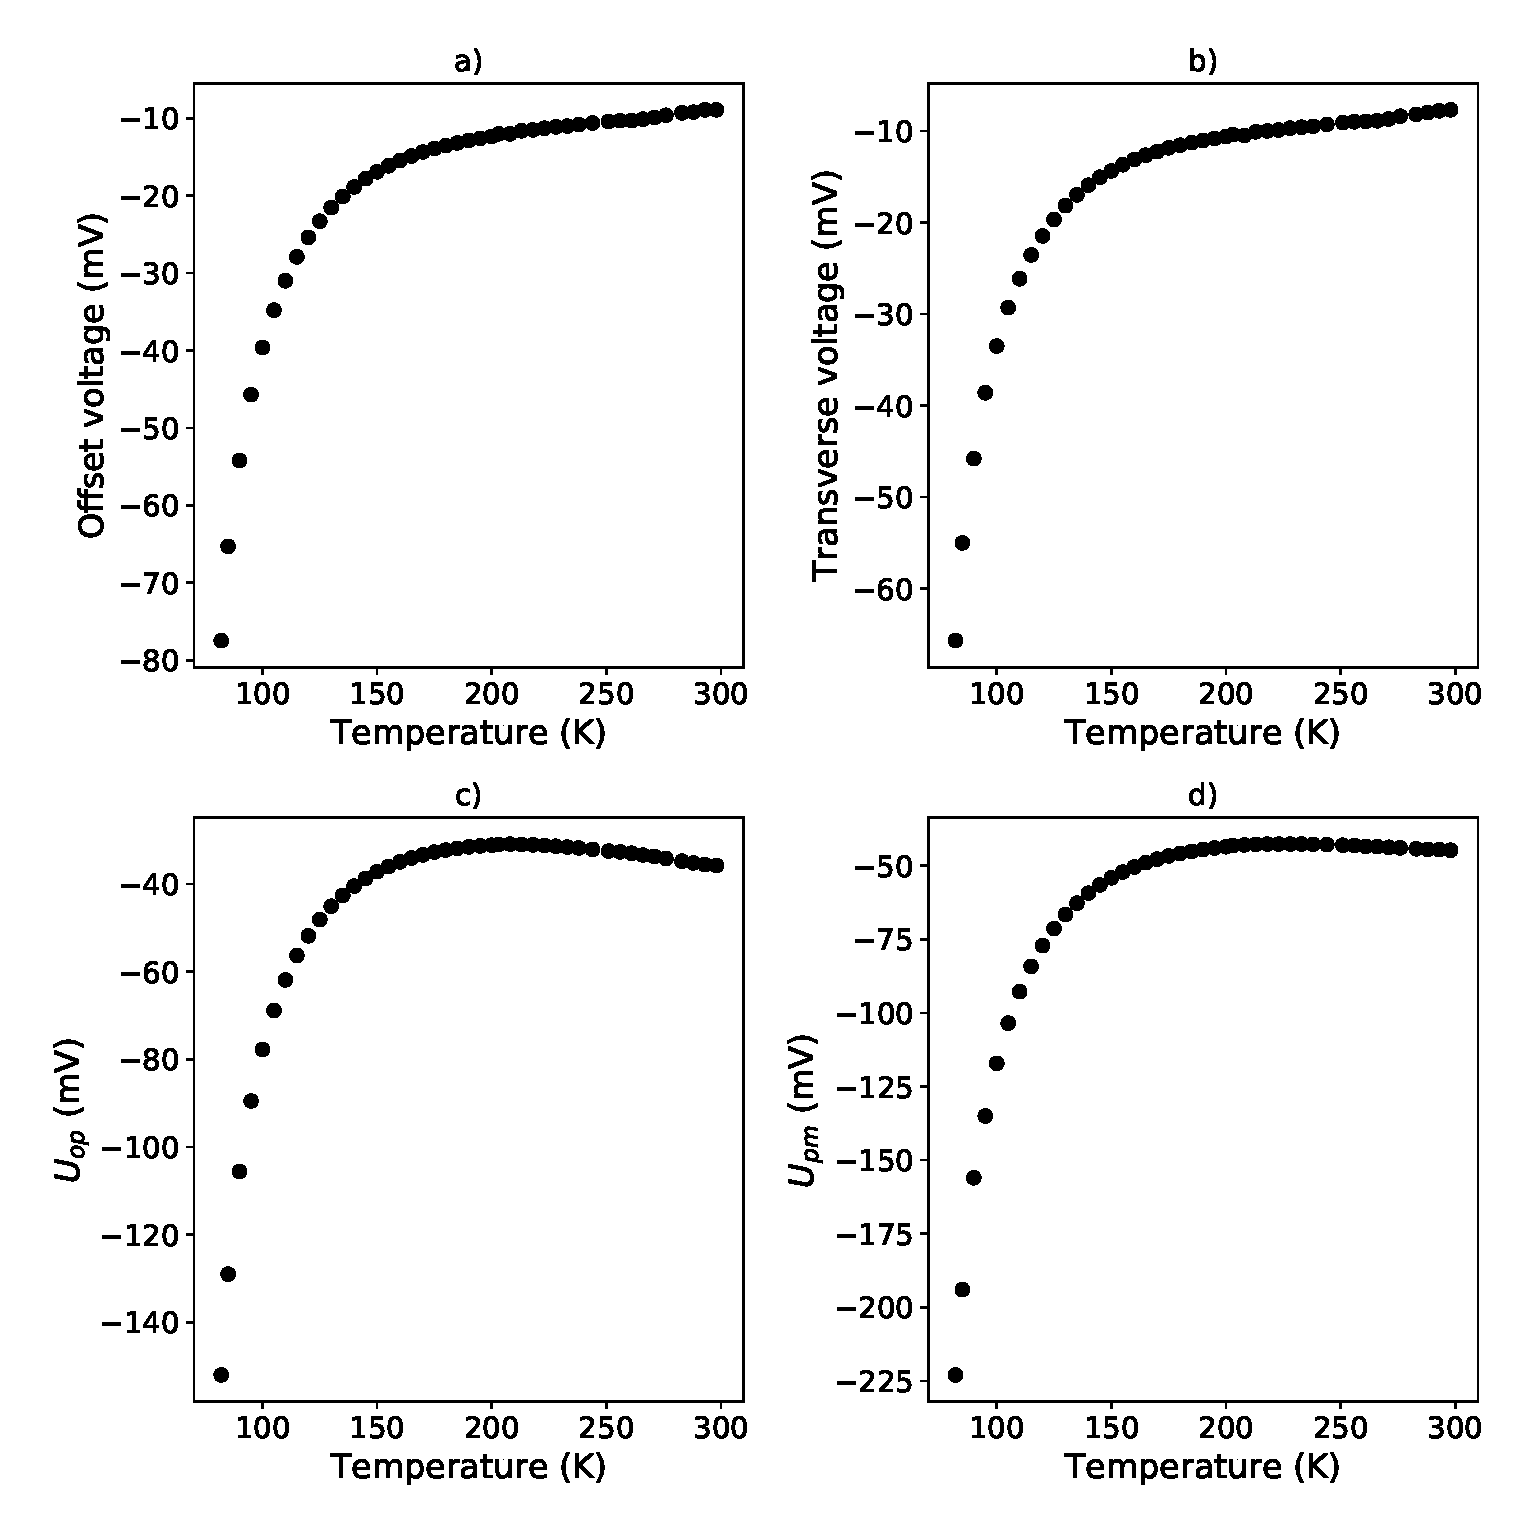
\includegraphics[width=\textwidth]{final_dataset.eps}
\caption{Final dataset with the combined measurements. The four measured quantities in the lab are plotted against the temperature: a) the offset voltage in absence of magnetic field, b) the total transverse voltage and c-d) the two voltages required to use the van der Pauw method.}
\label{fig:final_dataset}
\end{figure}

\end{appendices}

\end{document}